\documentclass{article}
\usepackage{graphicx}

\title{Tugas Database 2}
\author{Murnia Lestari}
\date{1184006}

\begin{document}

\maketitle
\section{Cara Membuat Aplikasi Builder dari file Excel ke Oracle Apex}
\begin{enumerate}
    \item Buka aplikasi Oracle Apex terlebih dahulu
         \begin{figure}[h]
            \centerline{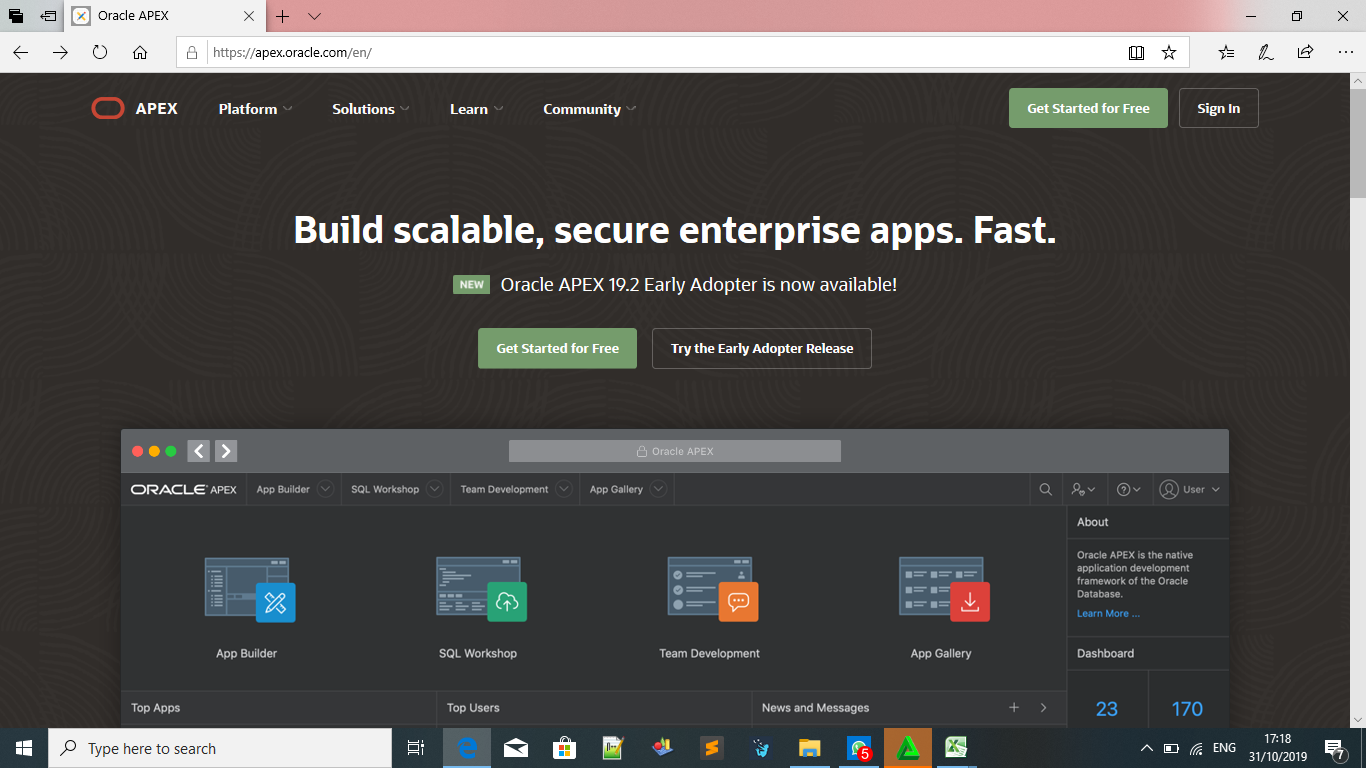
\includegraphics[width=8cm]{figure/sa.png}}
            \end{figure}
 \item Setelah itu masukkan workspace,username,dan password
         \begin{figure}[h]
    \centerline{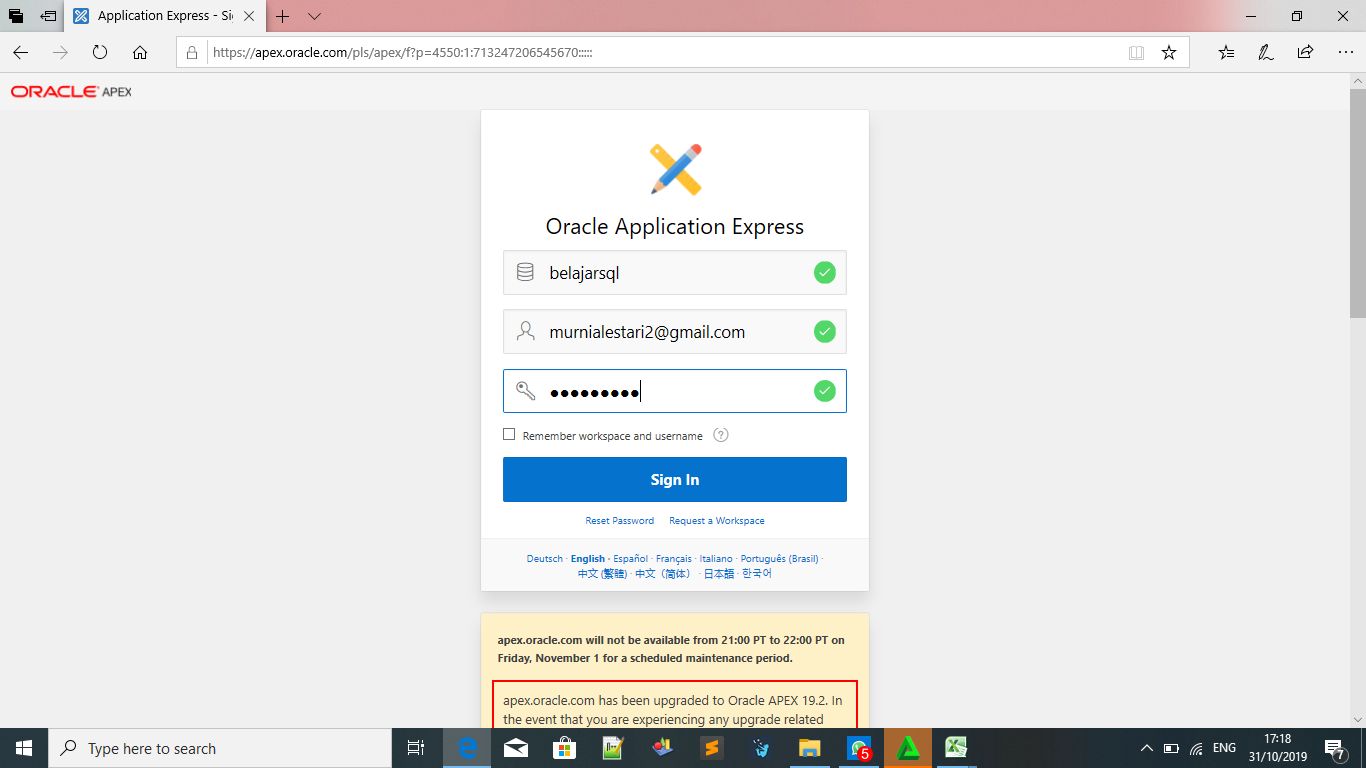
\includegraphics[width=8cm]{figure/su.png}}
       \end{figure}
      \newpage \item Setelah itu pilih App builder
    \begin{figure}[h]
    \centerline{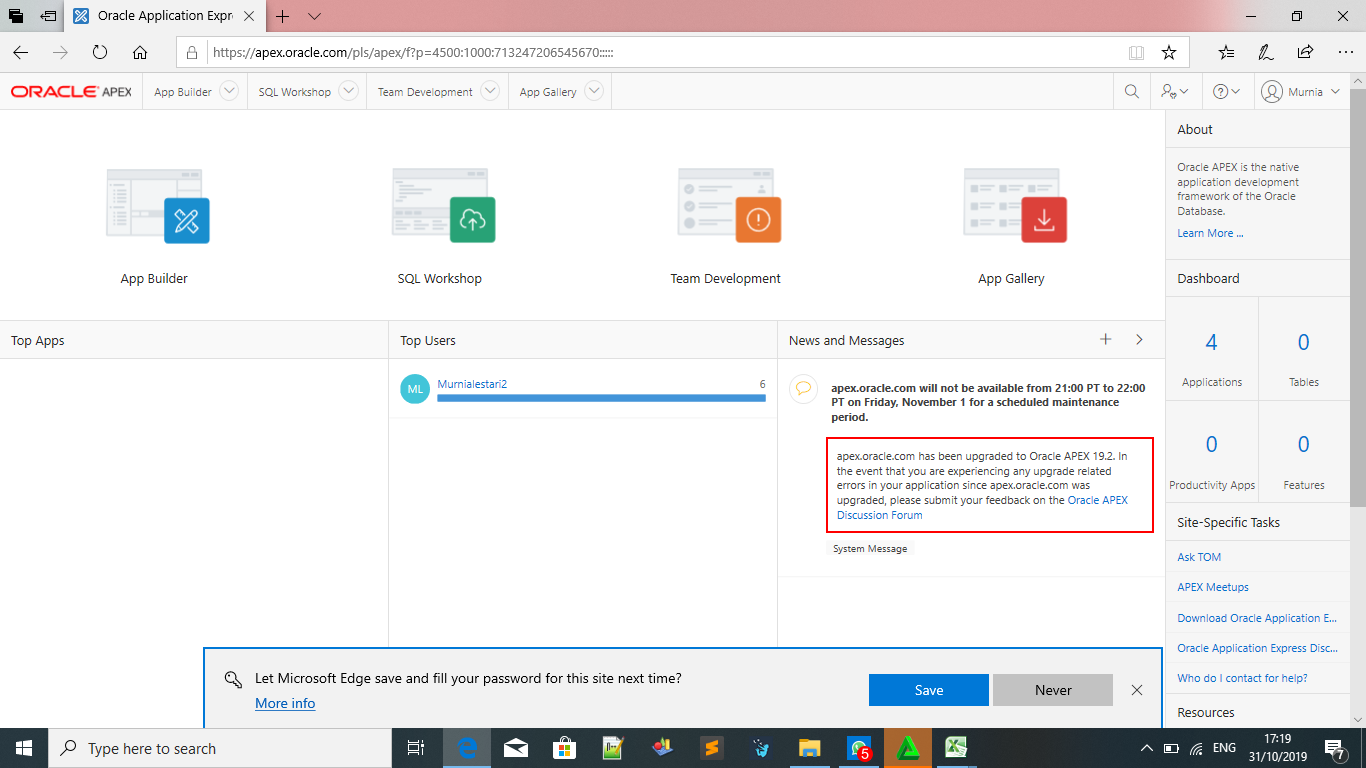
\includegraphics[width=8cm]{figure/bi.png}}
\end{figure}
  \item Setelah itu pilih create
    \begin{figure}[h]
  \centerline{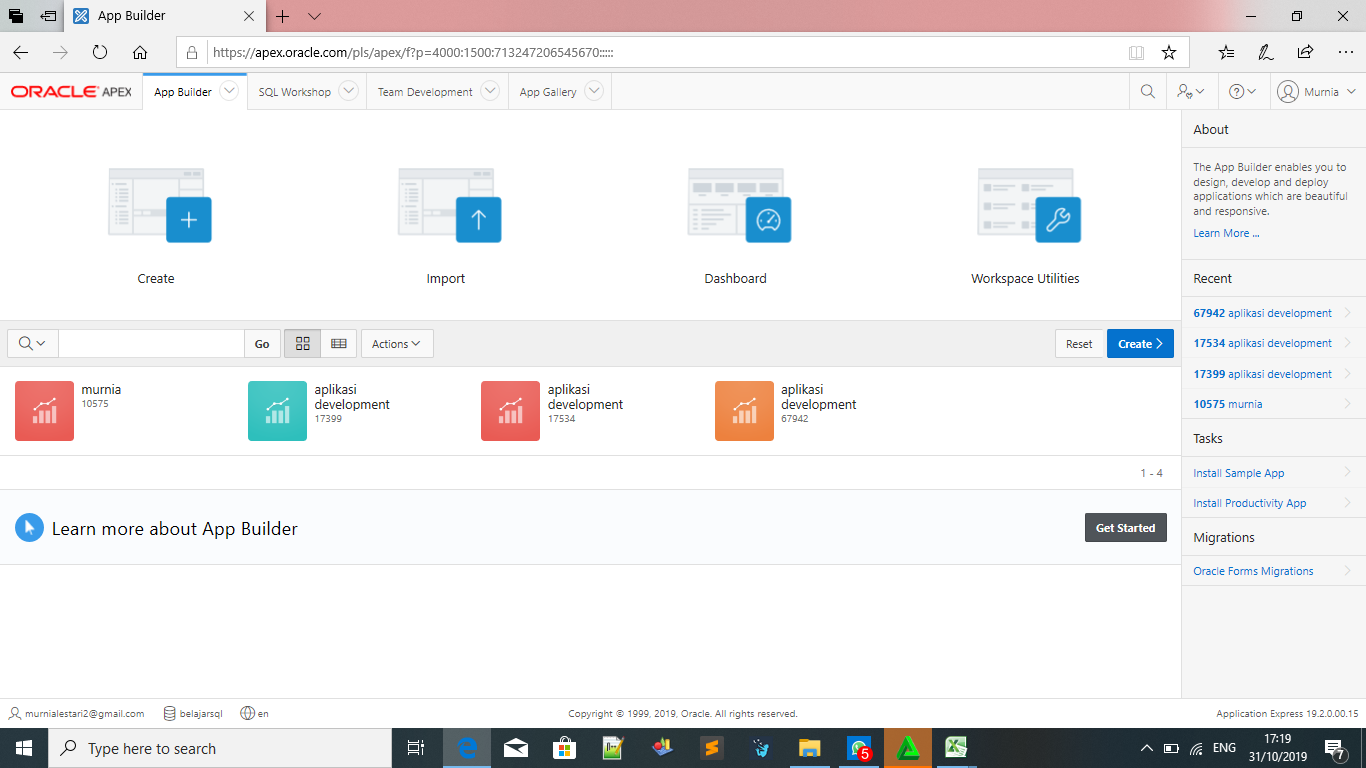
\includegraphics[width=8cm]{figure/la.png}}
\end{figure}
     \item Setelah itu pilih form a file
    \begin{figure}[h]
   \centerline{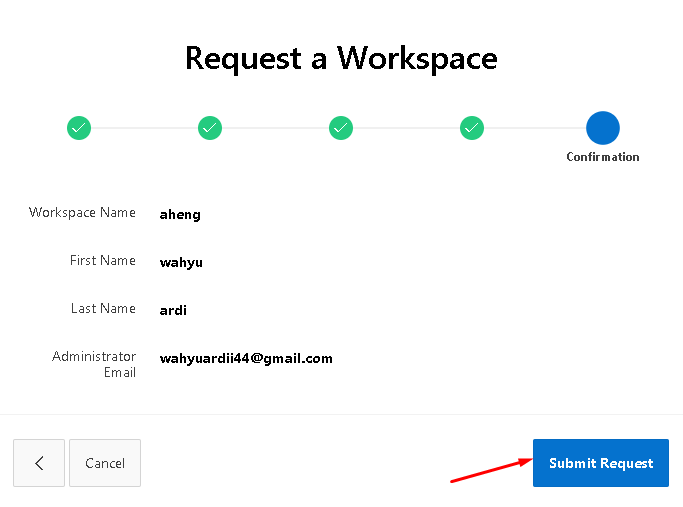
\includegraphics[width=8cm]{figure/g.png}}
   \end{figure}
\newpage\item lalu pilih file yang ingin kalian masukkan
    \begin{figure}[h]
   \centerline{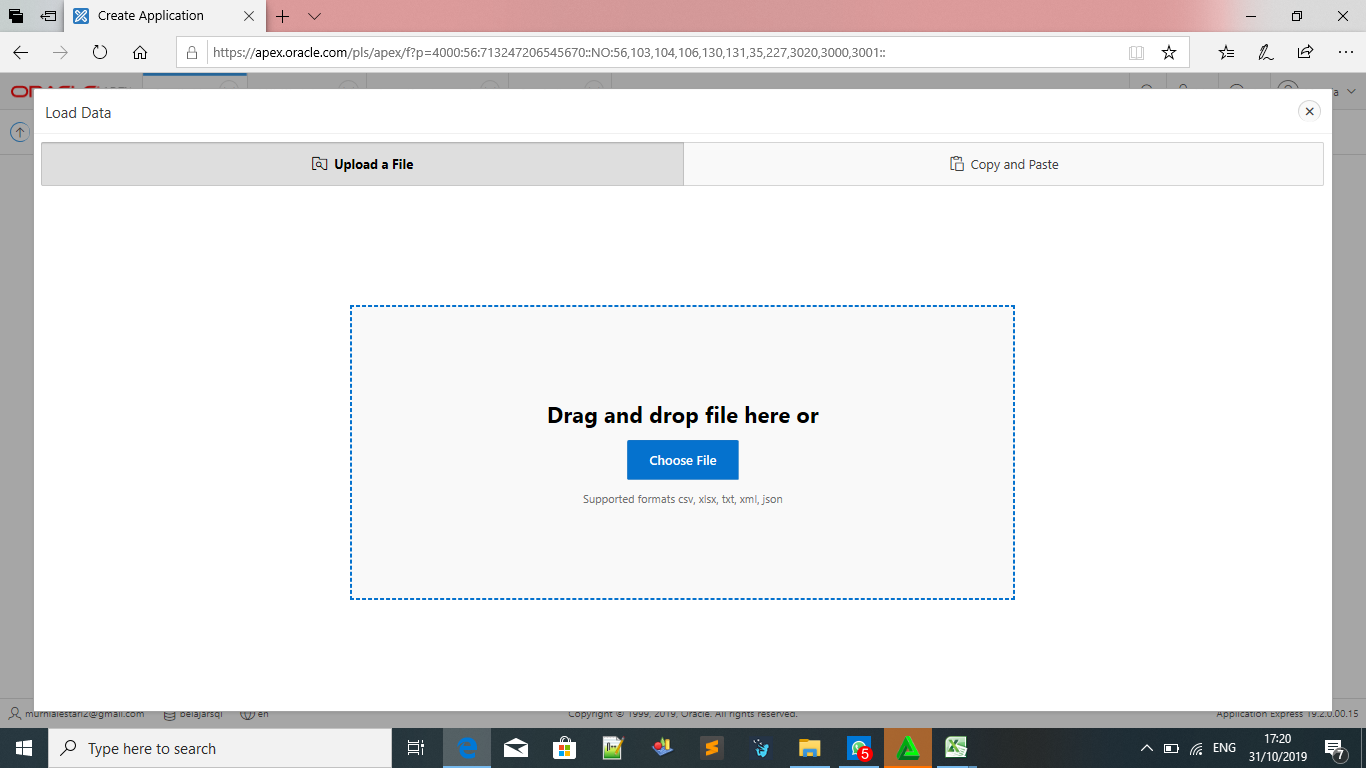
\includegraphics[width=8cm]{figure/li.png}}
\end{figure}
\newpage\item lalu masukkan nama table
    \begin{figure}[h]
   \centerline{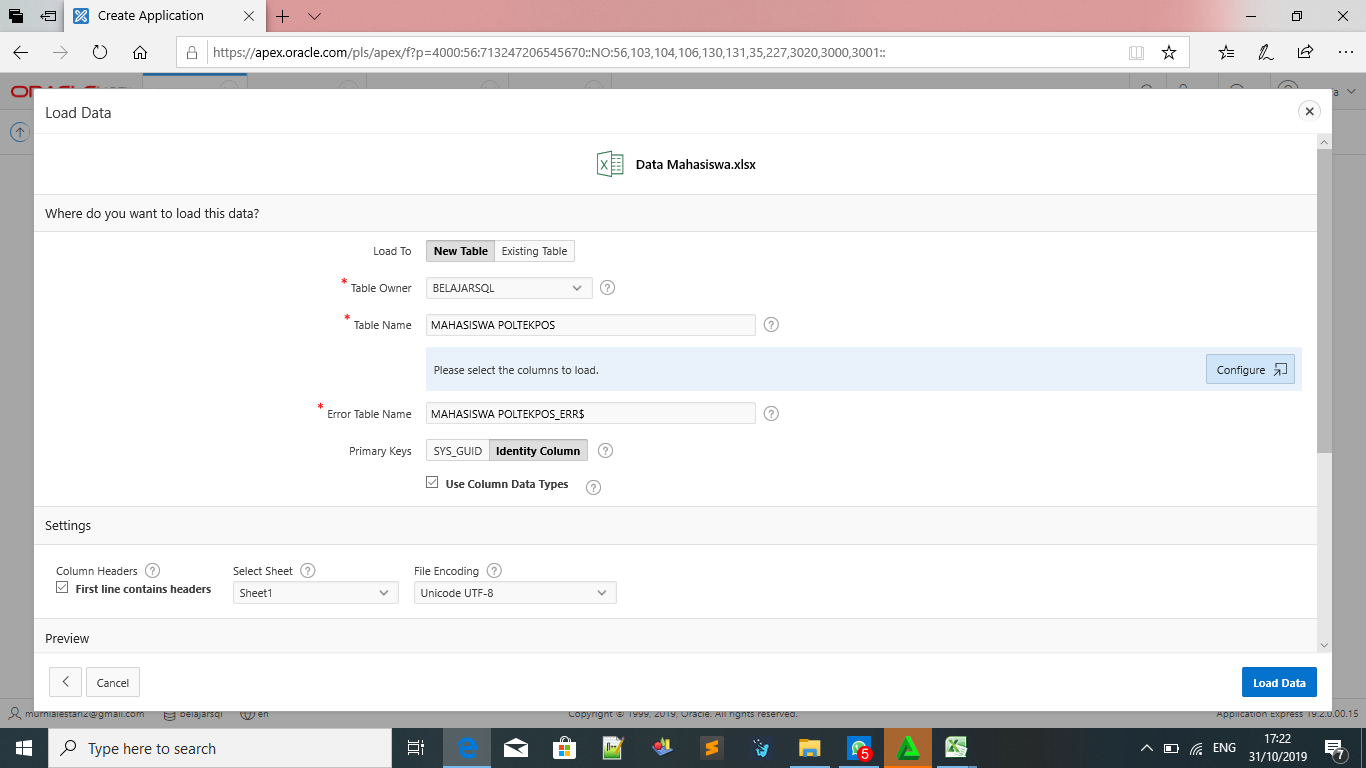
\includegraphics[width=8cm]{figure/lo.png}}
 \end{figure}
\item Setelah itu geser ke bawah,lalu pilih preview
    \begin{figure}[h]
   \centerline{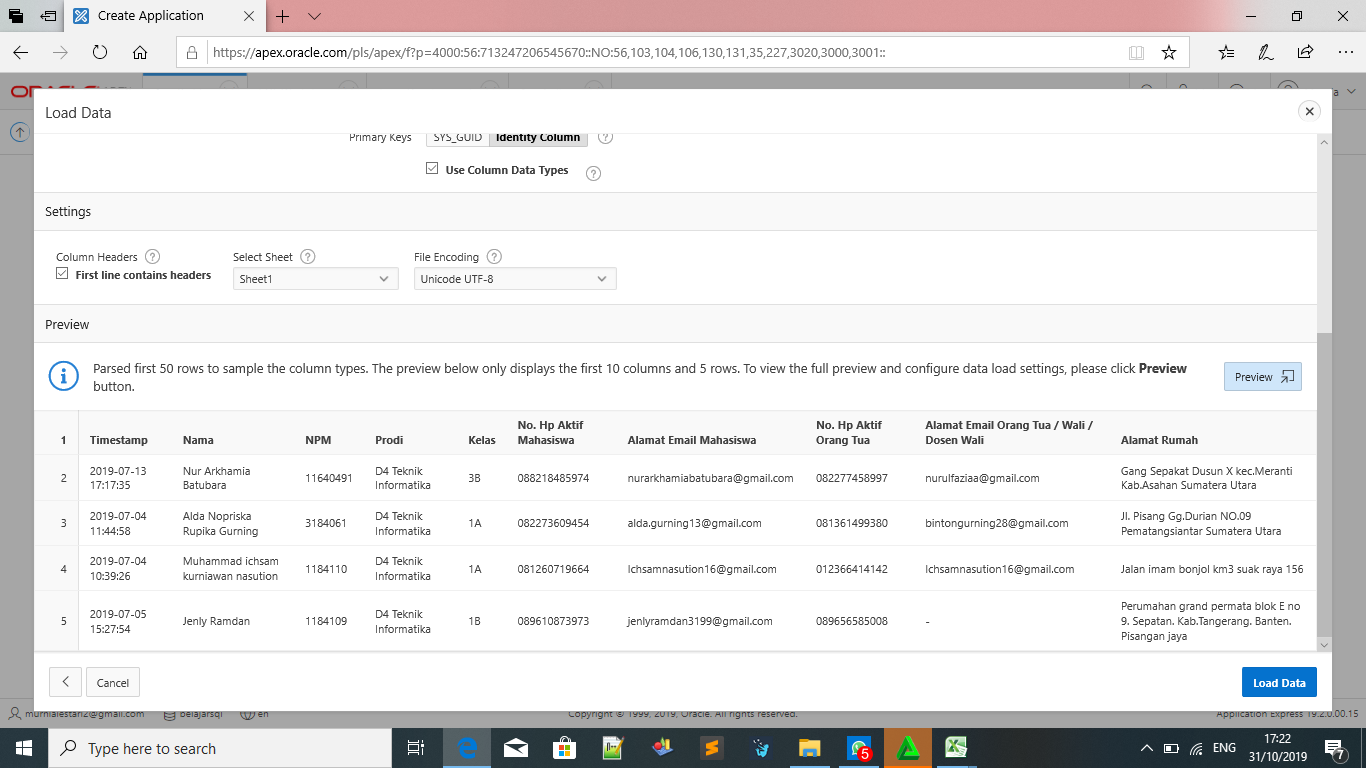
\includegraphics[width=8cm]{figure/le.png}}
\end{figure}
\newpage\item kalian bisa melihat data yang telah kalian masukkan
    \begin{figure}[h]
   \centerline{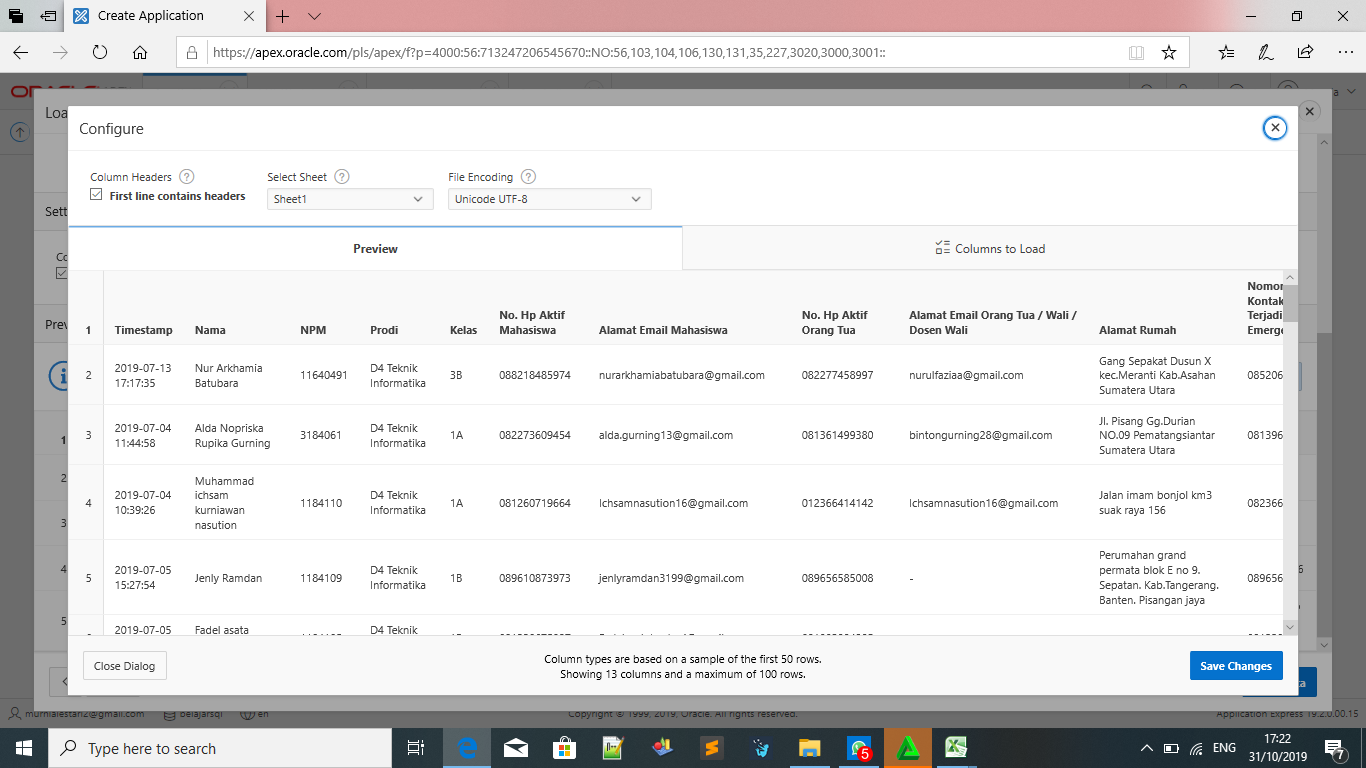
\includegraphics[width=8cm]{figure/se.png}}
\end{figure}
\item lalu pilih column to load untuk melihat nama column dan pilih save change
    \begin{figure}[h]
   \centerline{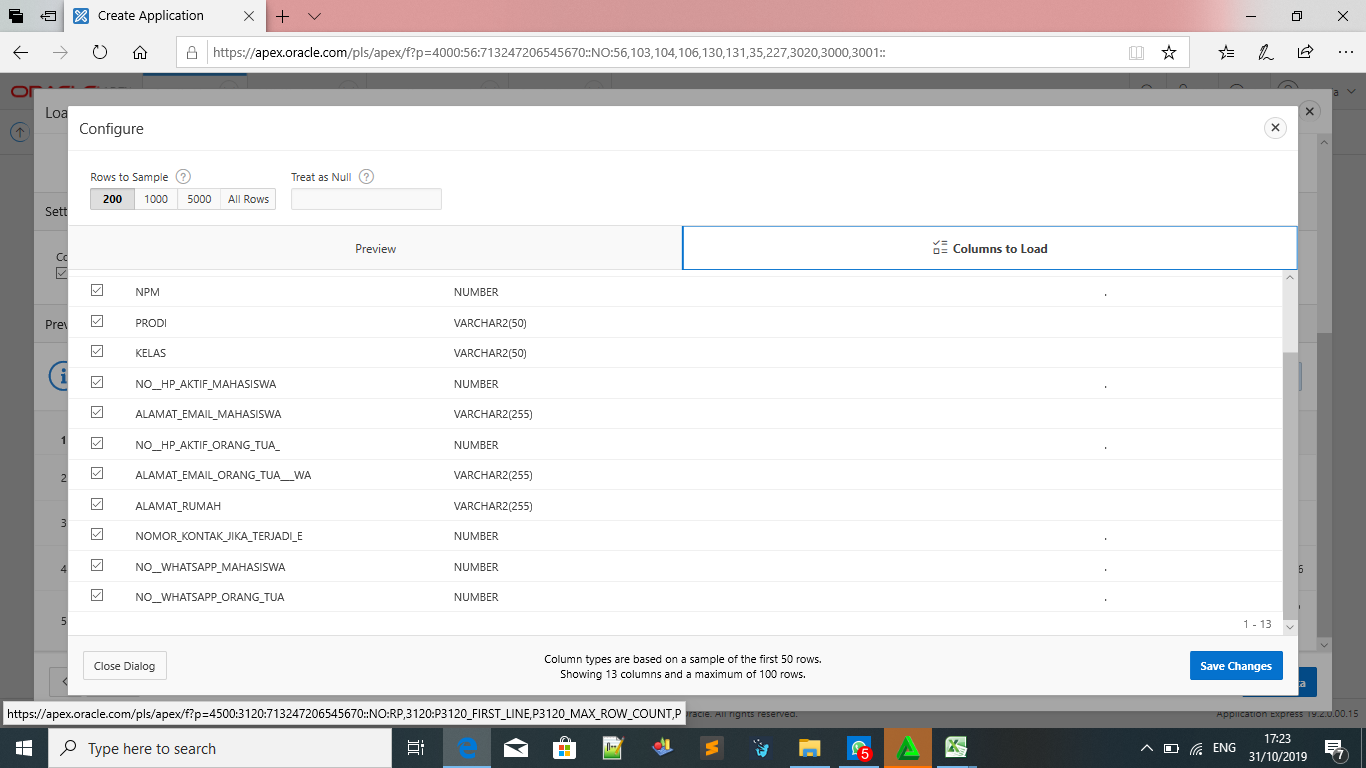
\includegraphics[width=8cm]{figure/de.png}}
\end{figure}
\newpage\item lalu pilih create aplication
    \begin{figure}[h]
   \centerline{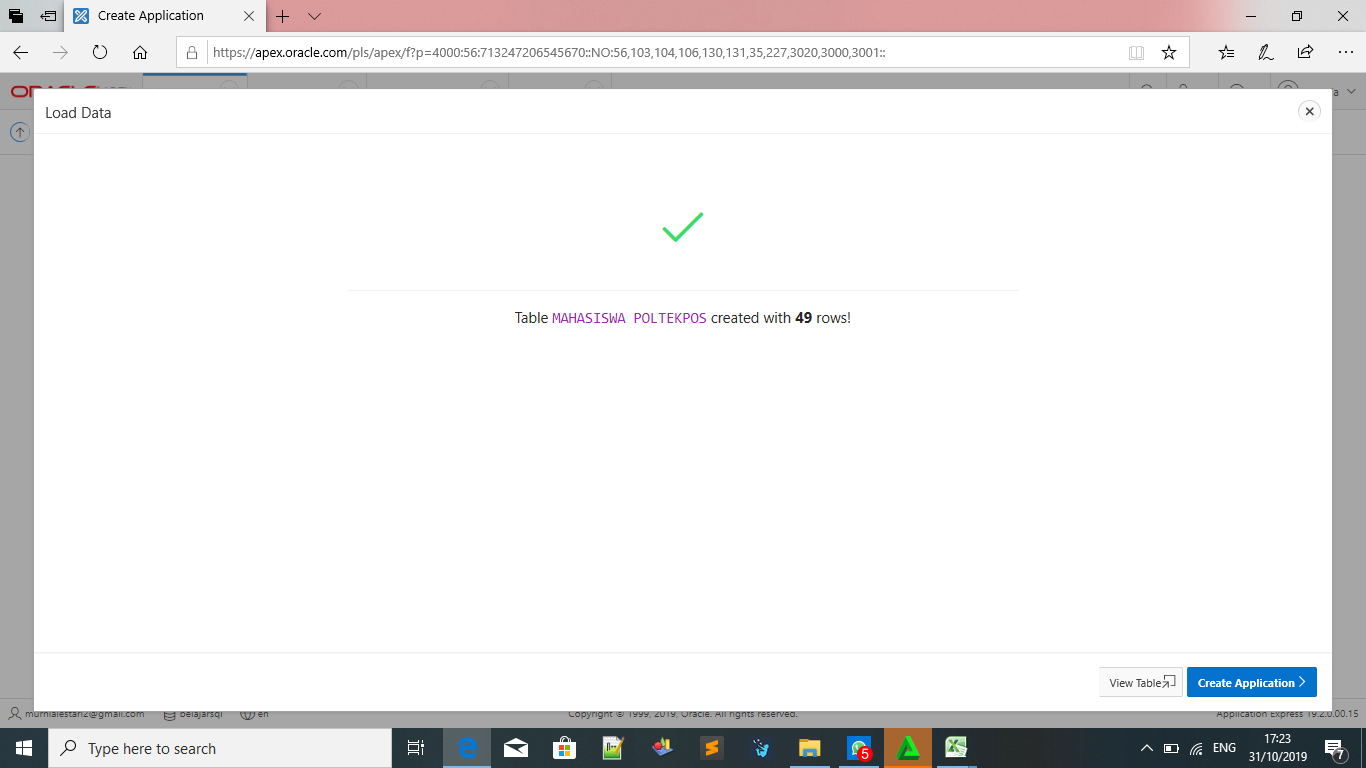
\includegraphics[width=8cm]{figure/di.png}}
\end{figure}
\item lalu pilih all pada features dan pilih create application
    \begin{figure}[h]
   \centerline{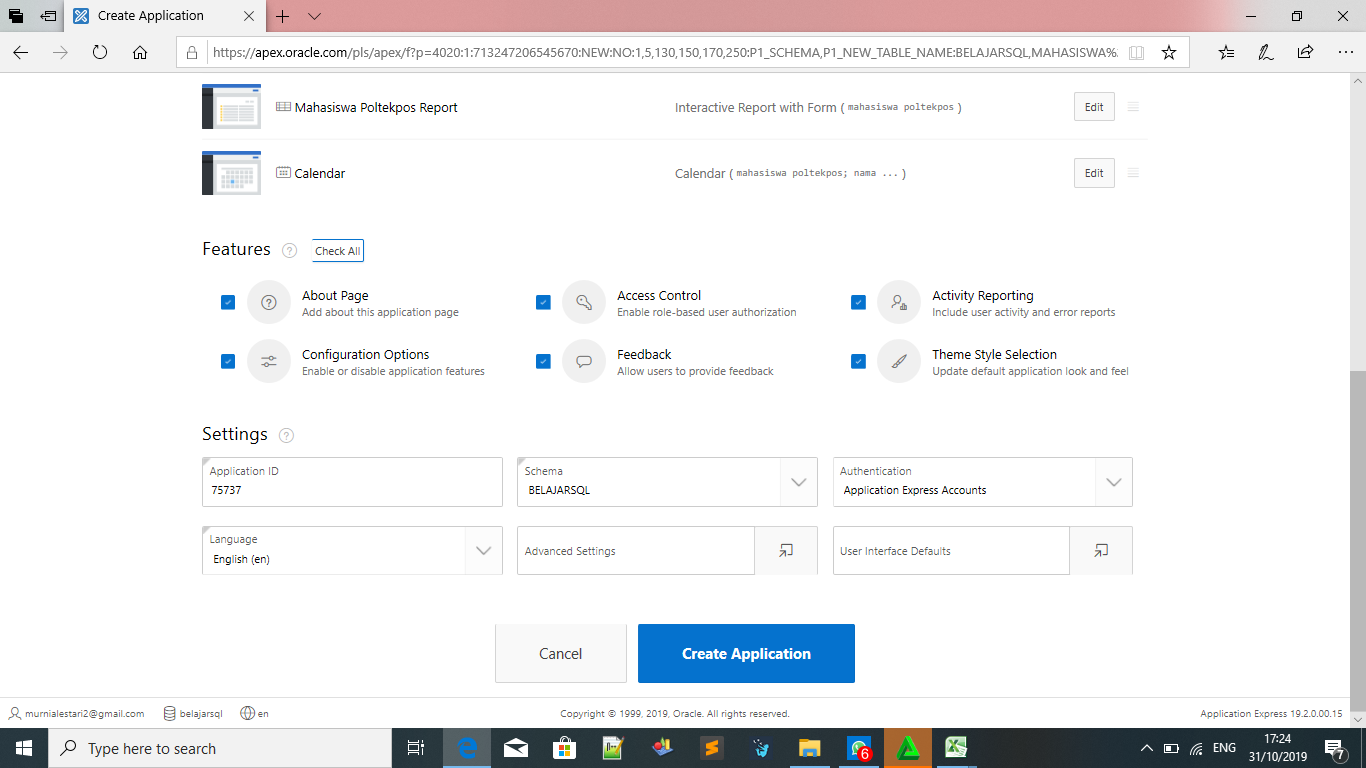
\includegraphics[width=8cm]{figure/da.png}}
\end{figure}
\newpage\item tunggu sampai selesai
    \begin{figure}[h]
   \centerline{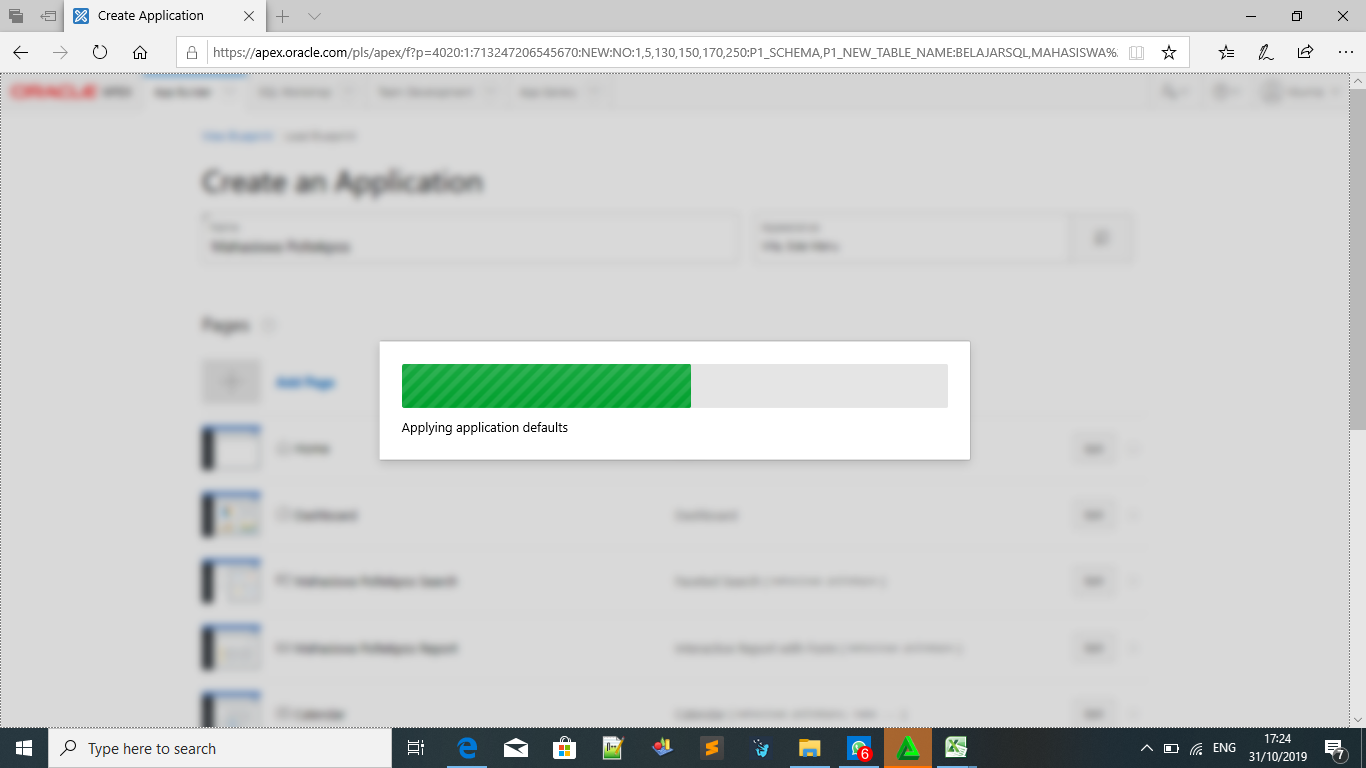
\includegraphics[width=8cm]{figure/ca.png}}
   \end{figure}
   \item lalu pilih run application
    \begin{figure}[h]
   \centerline{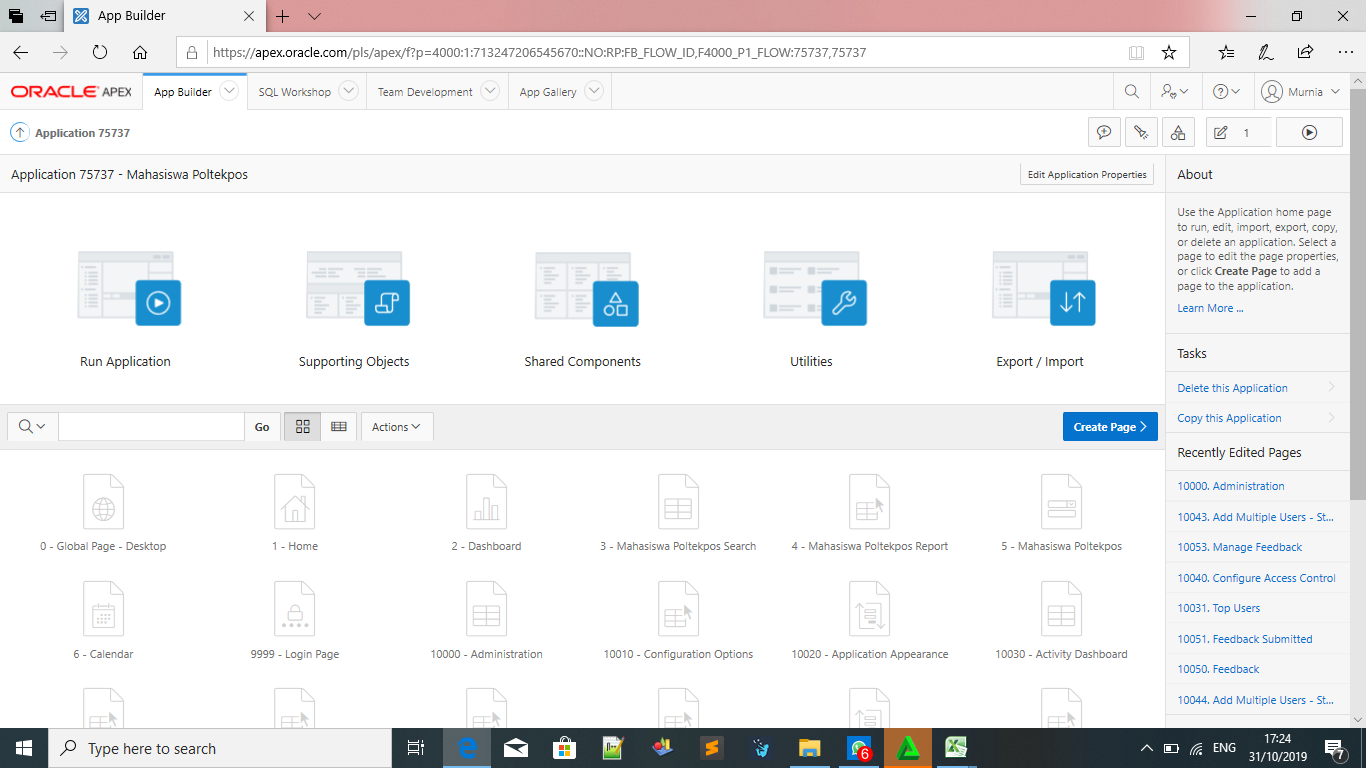
\includegraphics[width=8cm]{figure/c.png}}
\end{figure}
\newpage\item lalu masukkan username dan password
    \begin{figure}[h]
   \centerline{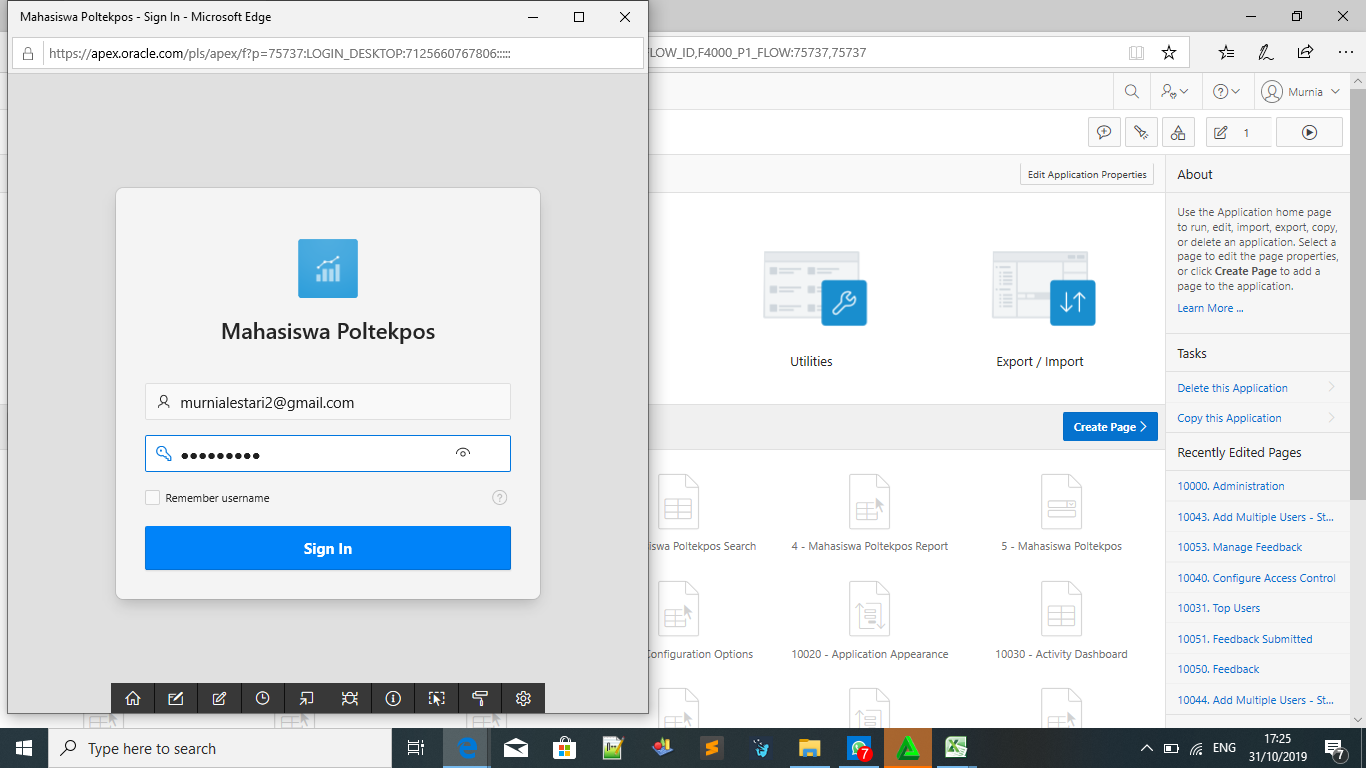
\includegraphics[width=8cm]{figure/ce.png}}
\end{figure}
\item lalu kalian bisa melihat tampilan aplikasi yang sudah jadi
    \begin{figure}[h]
   \centerline{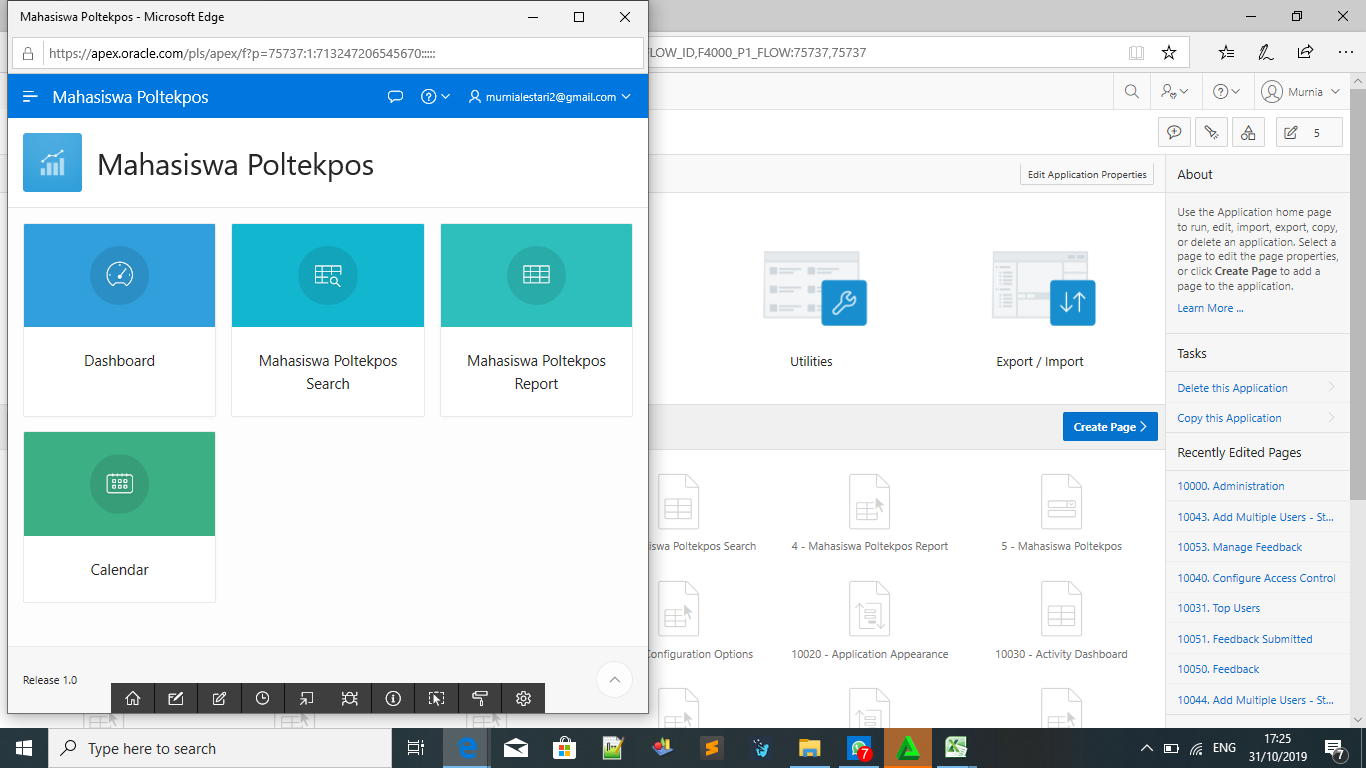
\includegraphics[width=8cm]{figure/ci.png}}
\end{figure}
\item berikut ini tampilan aplikasi yang sudah ada di dashboard
    \begin{figure}[h]
   \centerline{\includegraphics[width=8cm]{figure/capture.png}}
\end{figure}
\newpage\item berikut ini tampilan aplikasi yang sudah ada di mahasiswa poltekpos search
    \begin{figure}[h]
   \centerline{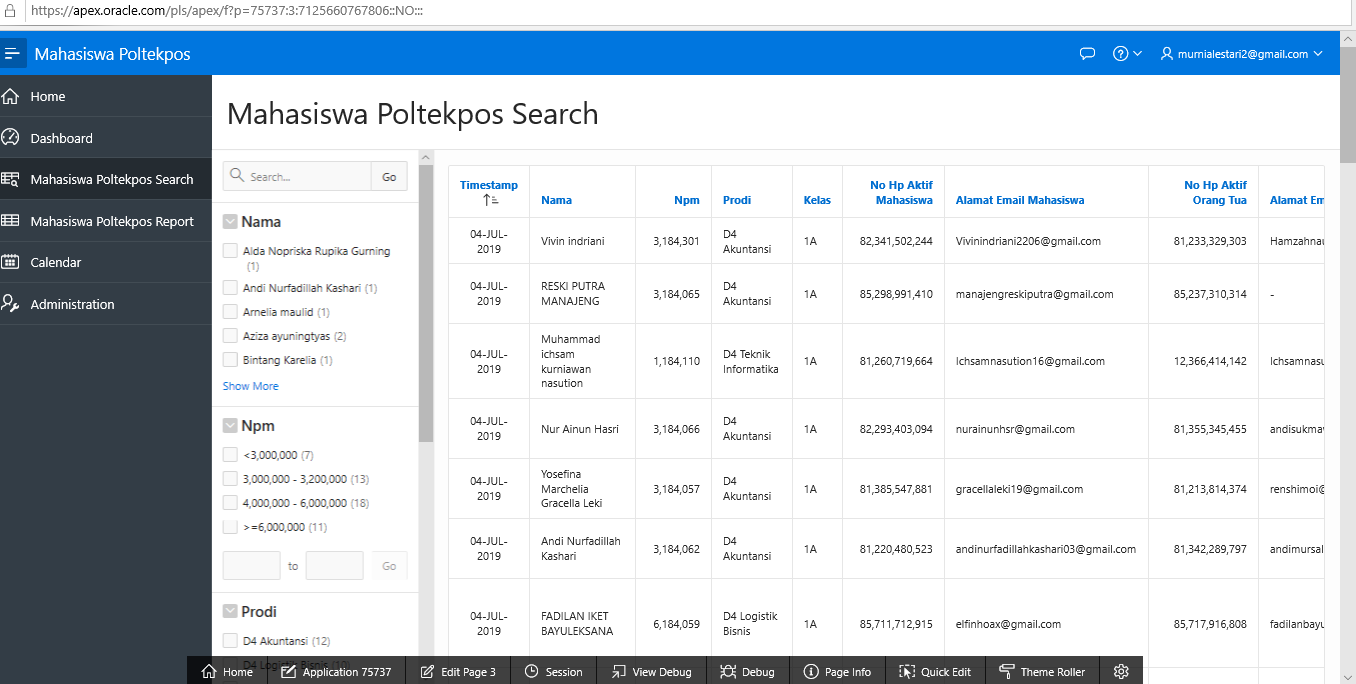
\includegraphics[width=8cm]{figure/ccc.png}}
\end{figure}
\item berikut ini tampilan aplikasi yang sudah ada di mahasiswa poltekpos report
    \begin{figure}[h]
   \centerline{\includegraphics[width=8cm]{figure/capture3.png}}
\end{figure}
\newpage\item berikut ini tampilan aplikasi yang sudah ada di calender
    \begin{figure}[h]
   \centerline{\includegraphics[width=8cm]{figure/capture4.png}}
\end{figure}
\item berikut ini tampilan administration
    \begin{figure}[h]
   \centerline{\includegraphics[width=8cm]{figure/capture5.png}}
\end{figure}
\end{enumerate}
\end{document}
